\documentclass{article}
\usepackage[a4paper, margin=2cm]{geometry}
\usepackage{xcolor}
\usepackage{xspace}
\usepackage{booktabs}
\usepackage{dsfont}
\usepackage{footmisc}
\usepackage{marvosym}
\usepackage{amsmath}
\usepackage{hyperref}
\usepackage[capitalise,noabbrev]{cleveref}
\usepackage{tabularx}
\usepackage{listings}
\usepackage{multirow}
\usepackage{pgfplots}
\pgfplotsset{compat=newest}

\usepgfplotslibrary{groupplots}
\pgfplotsset{every axis/.style={scale only axis}}

\pgfplotsset{
  major grid style={thin,dotted},
  minor grid style={thin,dotted},
  ymajorgrids,
  yminorgrids,
  every axis/.append style={
    line width=0.7pt,
    tick style={
      line cap=round,
      thin,
      major tick length=4pt,
      minor tick length=2pt,
    },
  },
  legend cell align=left,
  legend style={
    line width=0.7pt,
    /tikz/every even column/.append style={column sep=3mm,black},
    /tikz/every odd column/.append style={black},
  },
  % move title closer
  legend style={font=\small},
  title style={yshift=-2pt},
  % less space on left and right
  enlarge x limits=0.04,
  every tick label/.append style={font=\footnotesize},
  every axis label/.append style={font=\small},
  every axis y label/.append style={yshift=-1ex},
  /pgf/number format/1000 sep={},
  axis lines*=left,
  xlabel near ticks,
  ylabel near ticks,
  axis lines*=left,
  label style={font=\footnotesize},       
  tick label style={font=\footnotesize},
  plotBigComparison/.style={
    width=32.5mm,
    height=38.0mm,
  },
}

\title{PaCHash plot}
\date{}
\begin{document}
\definecolor{colorPaCHash}{HTML}{377EB8}
\definecolor{colorSeparator}{HTML}{000000}
\definecolor{colorPthash}{HTML}{000000}
\definecolor{colorLevelDb}{HTML}{FF7F00}
\definecolor{colorSilt}{HTML}{4DAF4A}
\definecolor{colorRocksDb}{HTML}{984EA3}
\definecolor{colorRecSplit}{HTML}{A65628}
\definecolor{colorUnorderedMap}{HTML}{F781BF}
\definecolor{colorCuckoo}{HTML}{E41A1C}
\definecolor{colorChd}{HTML}{444444}

\pgfplotscreateplotcyclelist{mycolorlist}{%
  {colorPaCHash, mark=diamond},
  {colorLevelDb, mark=square},
  {colorSilt, mark=o},
  {colorSeparator, mark=triangle},
  {colorRocksDb, mark=pentagon}
}
\pgfdeclareplotmark{pacman}{%
  \pgfpathmoveto{\pgfpointorigin}%
  \pgfpathlineto{\pgfqpointpolar{40}{1.2\pgfplotmarksize}}%
  \pgfpatharc{40}{320}{1.2\pgfplotmarksize}%
  \pgfpathlineto{\pgfpointorigin}%
  \pgfusepath{fill}
}
\pgfdeclareplotmark{flippedTriangle}{%
  \pgfpathmoveto{\pgfqpointpolar{-90}{1.2\pgfplotmarksize}}%
  \pgfpathlineto{\pgfqpointpolar{30}{1.2\pgfplotmarksize}}%
  \pgfpathlineto{\pgfqpointpolar{150}{1.2\pgfplotmarksize}}%
  \pgfpathclose%
  \pgfusepath{stroke}
}

% IMPORT-DATA competitorNames competitorNames.txt
% IMPORT-DATA objectStores comparisonPlot.txt

\begin{figure*}[t]
  \begin{tabular}{crrr}
    \multirow{-5}{*}{{\rotatebox[origin=c]{90}{\textbf{Fixed Size Objects}}}}
    &
    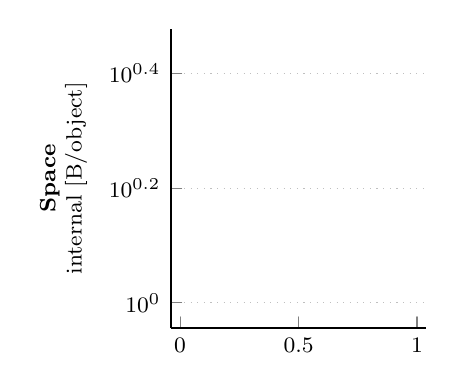
\begin{tikzpicture}
    \begin{axis}[
      plotBigComparison,
      ylabel={\begin{tabular}{c}\textbf{Space}\\internal [B/object]\end{tabular}},
      ymode=log,
      ]
      %% MULTIPLOT(store_name|ptitle|attr) SELECT
      %% numObjects/1000000.0 as x,
      %% 1.0*AVG(internalSpaceBytes)/numObjects as y,
      %% store_name as ptitle,
      %% attr,
      %% MULTIPLOT
      %% FROM objectStores
      %% JOIN competitorNames on method=store_code
      %% WHERE plots LIKE "%internal%"
      %% GROUP BY MULTIPLOT, x
      %% ORDER BY -sort_plot, MULTIPLOT, x

      \legend{};
    \end{axis}
  \end{tikzpicture}
  &
  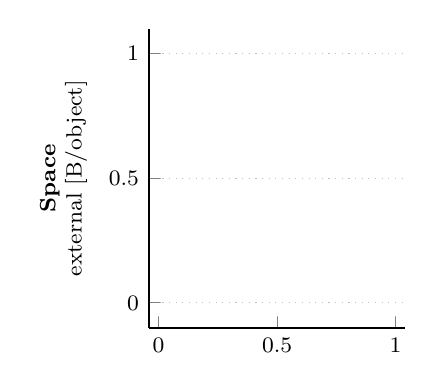
\begin{tikzpicture}
    \begin{axis}[
      plotBigComparison,
      ylabel={\begin{tabular}{c}\textbf{Space}\\external [B/object]\end{tabular}},
      ]
      %% MULTIPLOT(store_name|ptitle|attr) SELECT
      %% numObjects/1000000.0 as x,
      %% 1.0*AVG(externalSpaceBytes)/numObjects as y,
      %% store_name as ptitle,
      %% attr,
      %% MULTIPLOT
      %% FROM objectStores
      %% JOIN competitorNames on method=store_code
      %% WHERE plots LIKE "%external%"
      %% GROUP BY MULTIPLOT, x
      %% ORDER BY -sort_plot, MULTIPLOT, x

      \legend{};
    \end{axis}
  \end{tikzpicture}
  &
  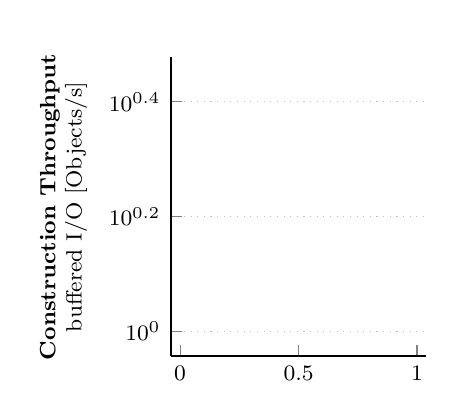
\begin{tikzpicture}
    \begin{axis}[
      plotBigComparison,
      ylabel={\begin{tabular}{c}\textbf{Construction Throughput}\\ buffered I/O [Objects/s]\end{tabular}},
      ymode=log,
      ]
      %% MULTIPLOT(store_name|ptitle|attr) SELECT
      %% numObjects/1000000.0 as x,
      %% 1.0*numObjects/(0.001*AVG(constructionTimeMs)) as y,
      %% store_name as ptitle,
      %% attr,
      %% MULTIPLOT
      %% FROM objectStores
      %% JOIN competitorNames on method=store_code
      %% WHERE plots LIKE "%construction%"
      %% GROUP BY MULTIPLOT, x
      %% ORDER BY -sort_plot, MULTIPLOT, x

      \legend{};
    \end{axis}
  \end{tikzpicture}
    \\
    &
  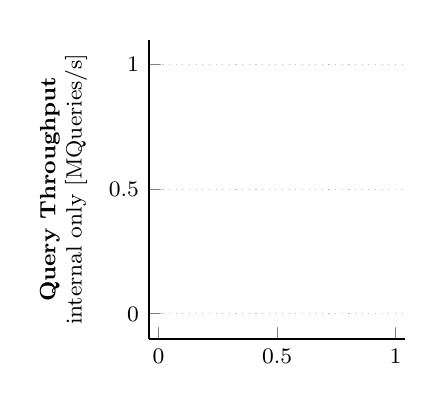
\begin{tikzpicture}
    \begin{axis}[
      plotBigComparison,
      ylabel={\begin{tabular}{c}\textbf{Query Throughput}\\internal only [MQueries/s]\end{tabular}},
      % xlabel={Number of objects [Millions]},
      ]
      %% MULTIPLOT(store_name|ptitle|attr) SELECT
      %% numObjects/1000000.0 as x,
      %% AVG(queriesPerSecond)/1000000 as y,
      %% store_name as ptitle,
      %% attr,
      %% MULTIPLOT
      %% FROM objectStores
      %% JOIN competitorNames on method=store_code
      %% WHERE plots LIKE "%index%"
      %% GROUP BY MULTIPLOT, x
      %% ORDER BY -sort_plot, MULTIPLOT, x

      \legend{};
    \end{axis}
  \end{tikzpicture}
  &
  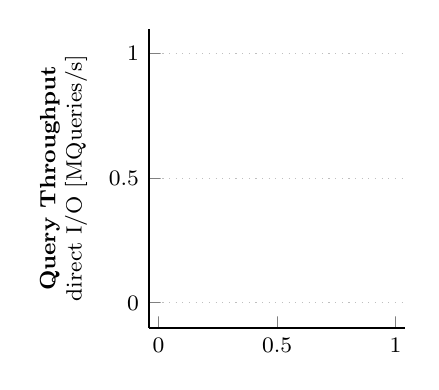
\begin{tikzpicture}
    \begin{axis}[
      plotBigComparison,
      %xlabel={Number of objects [Millions]},
      ylabel={\begin{tabular}{c}\textbf{Query Throughput}\\direct I/O [MQueries/s]\end{tabular}},
      ]
      %% MULTIPLOT(store_name|ptitle|attr) SELECT
      %% numObjects/1000000.0 as x,
      %% AVG(queriesPerSecond)/1000000 as y,
      %% store_name as ptitle,
      %% attr,
      %% MULTIPLOT
      %% FROM objectStores
      %% JOIN competitorNames on method=store_code
      %% WHERE plots LIKE "%direct%"
      %% GROUP BY MULTIPLOT, x
      %% ORDER BY -sort_plot, MULTIPLOT, x

      \legend{};
    \end{axis}
  \end{tikzpicture}
  &
  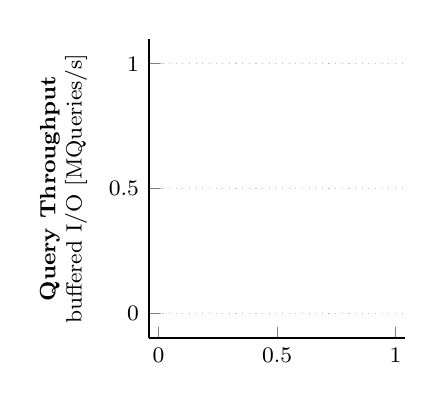
\begin{tikzpicture}
    \begin{axis}[
      plotBigComparison,
      % xlabel={Number of objects [Millions]},
      ylabel={\begin{tabular}{c}\textbf{Query Throughput}\\buffered I/O [MQueries/s]\end{tabular}},
      ]
      %% MULTIPLOT(store_name|ptitle|attr) SELECT
      %% numObjects/1000000.0 as x,
      %% AVG(queriesPerSecond)/1000000 as y,
      %% store_name as ptitle,
      %% attr,
      %% MULTIPLOT
      %% FROM objectStores
      %% JOIN competitorNames on method=store_code
      %% WHERE plots LIKE "%buffered%"
      %% GROUP BY MULTIPLOT, x
      %% ORDER BY -sort_plot, MULTIPLOT, x

      \legend{};
    \end{axis}
  \end{tikzpicture}
  \end{tabular}
  \vspace{-.1cm}
  \begin{center}
  \begin{tikzpicture}
    \begin{axis}[
      legend pos=north west,
      width=4cm,
      height=2cm,
      hide axis,
      xmin=10,
      xmax=50,
      ymin=0,
      ymax=0.4,
      legend style={font=\small},
      legend columns=3,
      transpose legend,
      % transpose legend,
      % legend columns=4,
      % legend to name={leg:big_comparison_table},
      ]
      %% MULTIPLOT(store_name|ptitle|attr) SELECT
      %% 0 as x, 0 as y,
      %% store_name as ptitle,
      %% attr, MULTIPLOT
      %% FROM competitorNames
      %% WHERE plots LIKE "%legend%"
      %% ORDER BY sort_legend, MULTIPLOT
      \addplot[color=colorChd,mark=oplus,densely dotted,mark options={solid}] coordinates { (0,0) };
      \addlegendentry{CHD (16-perfect)};
      \addplot[color=colorCuckoo,mark=+,densely dotted,mark options={solid}] coordinates { (0,0) };
      \addlegendentry{Cuckoo (here)};
      \addplot[color=colorLevelDb,mark=o] coordinates { (0,0) };
      \addlegendentry{LevelDB};
      \addplot[color=colorLevelDb,mark=triangle] coordinates { (0,0) };
      \addlegendentry{LevelDB (Static part)};
      \addplot[color=colorPthash,mark=|,densely dotted,mark options={solid}] coordinates { (0,0) };
      \addlegendentry{PTHash };
      \addplot[color=colorPaCHash,mark=pacman] coordinates { (0,0) };
      \addlegendentry{PaCHash (here)};
      \addplot[color=colorRecSplit,mark=x,densely dotted,mark options={solid}] coordinates { (0,0) };
      \addlegendentry{RecSplit};
      \addplot[color=colorRocksDb,mark=diamond] coordinates { (0,0) };
      \addlegendentry{RocksDB};
      \addplot[color=colorSilt,mark=square,densely dotted,mark options={solid}] coordinates { (0,0) };
      \addlegendentry{SILT};
      \addplot[color=colorSilt,mark=otimes,densely dotted,mark options={solid}] coordinates { (0,0) };
      \addlegendentry{SILT (Static part)};
      \addplot[color=colorSeparator,mark=flippedTriangle,densely dotted,mark options={solid}] coordinates { (0,0) };
      \addlegendentry{Separator (here)};
      \addplot[color=colorUnorderedMap,mark=pentagon] coordinates { (0,0) };
      \addlegendentry{std::unordered\_map};
    \end{axis}
  \end{tikzpicture}
  \end{center}
  \vspace{-.8cm}
  \caption{Comparison with competitor object stores using objects of fixed size 256 bytes.
  Keys are 8 byte random strings.
  Dotted lines indicate methods supporting only objects of identical size natively.
  We enhanced two of them to partially support variable size objects.}
  \label{fig:competitors}
\end{figure*}

\end{document}

